\chapter{Eigener Ansatz}

\section{Zielsetzung}
Die vorliegende Arbeit handelt davon mit Hilfe eines eigens erstellten 3D Modells eine Drohne Indoor navigieren zu können. Um dies umsetzen zu können gibt es einen Quadrokopter der zu diesem Zwecke eingesetzt werden kann. \\
Heutzutage basiert die Navgiation vieler Drohnen auf \ac{GPS} allerdings kann man Drohnen innerhalb von Gebäuden nicht mit dieser Technik fliegen lassen, da damit die im Innenraum vorhandenen Hindernisse nicht berücksichtigt werden können. Aus diesem Grund soll hierfür eine Möglichkeit gefunden werden, welche es ermöglicht, eine Drohne ohne \ac{GPS} im Innenraum eines Gebäudes mit Hilfe eines 3D Modells navigieren zu können.\\
Der Quadrokopter, die Coex Clover Drohne ist bereits mit verschiedenen Sensoren ausgestattet und kann potenziell mit weiteren Sensoren erweitert werden. Jedoch ist die Drohne bis zum Beginn dieser Arbeit noch nicht richtig geflogen ist. Somit muss zum einen die Nutzbarkeit der Drohne für dieses Projekt sichergestellt werden, um diese in dieser Arbeit einsetzen zu können. \\
Ziel dieser Arbeit ist es, bestenfalls den bereits vorhandenen Quadrokopter mit Hilfe eines eigens erstellten 3D Umweltmodells innerhalb eines Raumes navigieren zu können und dadurch kleinere Aufgaben wie beispielsweise das Auslesen eines QR-Codes somit erledigen zu können.



\section{Vorgehensweise}

In Abbildung \ref{fig:vorgehensweise} sind die 2 Vorgehensweisen die wir uns ausgedacht haben ersichtlich. In Ansatz 1 hatten wir zuerst versucht ein vorher gescanntes 3D Modell auf die Drohne zu laden und eine Positionierung im 3D Modell durchzuführen. Schnell wurde ersichtlich, dass es wenig sinnvoll eine Positionierung in einem vorher bekannten 3D Modell durchzuführen, da die Drohne auch in unbekannten Umgebungen eingesetzt werden soll. Deshalb ist es sinnvoller die Positionierung und die 3D Modell Erstellung zu kombinieren. Dazu kann \ac{SLAM} eingesetzt werden. Deshalb haben wir Ansatz 1 relativ schnell wieder verworfen.

\begin{figure}
    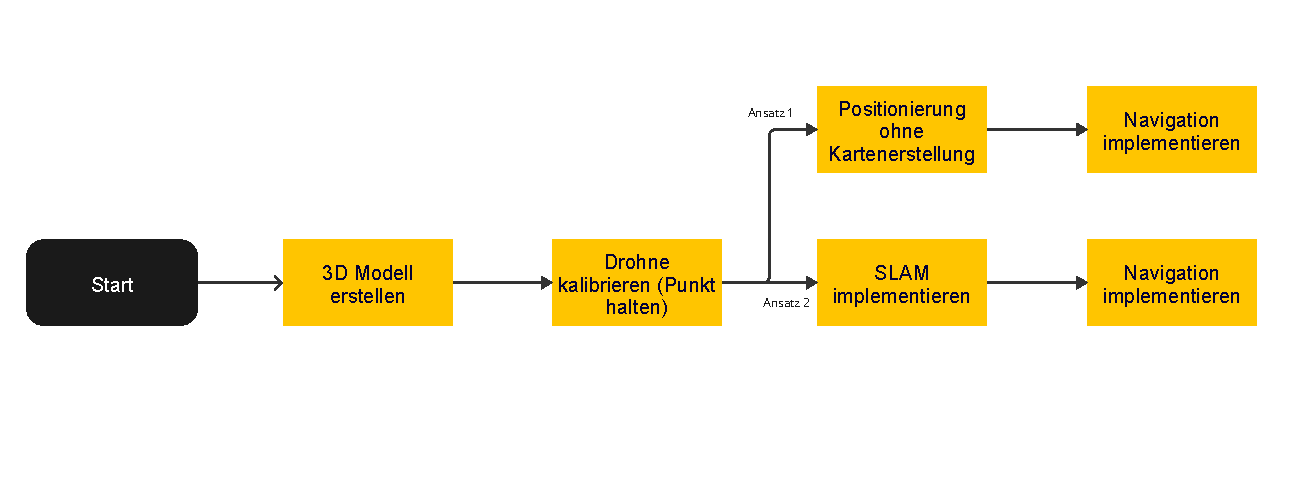
\includegraphics[scale=0.7]{images/ansatz_plan.pdf}
    \caption{Geplante Vorgehensweise}\label{fig:vorgehensweise}
\end{figure}

\subsection{Auswahl SLAM Algorithmus}

Es wurden mehrere \ac{SLAM}-Algorithmen in Betracht gezogen, und aufgrund der begrenzten Leistung des Raspberry Pi haben wir den Algorithmus mit den geringsten Anforderungen ausgewählt. Eine Übersicht der gebräuchlichen \ac{SLAM} Algorithmen ist in \ref{chp:übersicht-slamalgo} zu sehen.Für eine fundierte Auswahl wurde eine gewichtete Analyse erstellt, um den für unsere Zwecke bestens geeigneten \ac{SLAM} Algorithmus zu verwenden. Die Gewichte sehen Sie in Tabelle \ref{tab:vergleich-gewichtung-slam}, die Kriterien in \ref{tab:vergleich-kriterien-slam} und das Ergebnis in \ref{tab:vergleich-slam}

Bei der Bewertung von SLAM-Algorithmen gibt es mehrere Punkte, die zur Messung der Qualität und Eignung eines SLAM-Verfahrens herangezogen werden können.

\begin{description}
    \item[Genauigkeit]{Die Genauigkeit eines SLAM-Algorithmus bezieht sich darauf, wie genau die geschätzten Positionen und Kartendarstellungen mit den tatsächlichen Werten übereinstimmen. Eine höhere Genauigkeit ist für eine präzise Navigation und Kartierung wünschenswert}
    \item[Robustheit]{SLAM-Algorithmen sollten robust gegenüber Schwankungen in der Umgebung sein und mit schwierigen Bedingungen wie dynamischen Objekten, Verdeckungen oder Beleuchtungsänderungen umgehen können. Ein robuster Algorithmus behält selbst bei diesen Faktoren genaue Schätzungen bei} 
    \item[Skalierbarkeit]{Skalierbarkeit ist wichtig, wenn es um groß angelegte Kartierungsszenarien oder lang andauernde Operationen geht. Ein Algorithmus sollte in der Lage sein, wachsende Datenmengen zu verarbeiten, z. B. größere Umgebungen oder längere Einsatzzeiten, ohne dass die Leistung signifikant abnimmt}
    \item[Leistung in Echtzeit]{Die Echtzeitfähigkeit ist für viele Anwendungen entscheidend, insbesondere in der Robotik oder der erweiterten Realität. SLAM-Algorithmen sollten in der Lage sein, Sensordaten zu verarbeiten und Schätzungen in Echtzeit zu aktualisieren, um zeitnahe und reaktionsfähige Informationen zu liefern}
    \item[Berechnungseffizienz]{SLAM-Algorithmen sollten rechnerisch effizient sein, insbesondere bei ressourcenbeschränkten Plattformen wie dem Raspberry Pi. Es ist wichtig, einen Algorithmus zu wählen, der ein ausgewogenes Verhältnis zwischen Genauigkeit und Rechenanforderungen herstellt und eine optimale Leistung auf der gewählten Hardware gewährleistet}
    \item[Fähigkeit zur Sensorfusion]{Die Integration mehrerer Sensoren, wie z. B. Kameras, Inertialmesseinheiten (IMUs) oder Tiefensensoren, kann die SLAM-Leistung verbessern. Algorithmen, die Informationen von verschiedenen Sensoren effektiv fusionieren können, liefern oft genauere und zuverlässigere Ergebnisse}
    \item[Kartendarstellung]{Die Qualität und Darstellung der erzeugten Karte kann ebenfalls ein wichtiger Faktor sein. Ein guter SLAM-Algorithmus sollte Karten erzeugen, die geometrisch konsistent, visuell informativ und für nachfolgende Aufgaben oder Analysen nützlich sind} 
\end{description}

Zur Bewertung der \ac{SLAM} Algorithmen haben wir folgende Messungen als Referenz genommen \cite{ragot:hal-04071273} und \cite{Merzlyakov2021}

\subsection{Übersicht \ac{VSLAM} Algorithmen}

Da die Azure Kinect in dieser Arbeit verwendet sollen, werden alle \ac{SLAM} Verfahren, die nur mit monokular funktionierenden Kameras verwendet werden können ausgeschlossen.
Ansonsten kann der Depth \ac{ToF} Sensor der Azure Kinekt nicht verwendet werden. Im Vergleich aus der Arbeit von \citeauthor{Merzlyakov2021} kommen dann nur ORB-SLAM

\subsubsection{ElasticFusion}


ElasticFusion ist eine dichte SLAM-Methode, die RGB-D-Kameras verwendet. Es konstruiert ein global konsistentes Modell der Umgebung zur Verwendung in Roboteranwendungen wie Objekterkennung und -manipulation und bestimmt gleichzeitig die Sensorposition in Echtzeit. Erreicht wird dies durch eine Kombination aus Frame-to-Model-Kameratracking und oberflächenbasierter Fusion, die eine häufige Modellverfeinerung durch nicht starre Oberflächendeformationen nutzt.


\subsubsection{RTAB-Map}

RTAB-Map (Real-Time Appearance-Based Mapping) ist ein beliebter Open-Source SLAM-Algorithmus, der auf RGB-D, Stereo und \ac{Lidar} basiert. Er ist speziell für die langfristige und großflächige Kartierung von Umgebungen konzipiert. Das Hauptmerkmal von RTAB-Map ist seine Fähigkeit, Schleifenabschlüsse zu erkennen und zu verarbeiten, um eine genaue Kartierung über lange Zeiträume und Entfernungen aufrechtzuerhalten.

RTAB-Map verwendet eine Speicherverwaltungstechnik, um die kartierten Umgebungen zu verfolgen, wobei ein Kurzzeitspeicher für die jüngsten Beobachtungen und ein Langzeitspeicher für den Rest verwendet wird. Dies hilft bei der Bewältigung der Herausforderungen bei der Abbildung großer Umgebungen und beim Umgang mit Schleifenschlüssen. Außerdem verfügt es über einen Graph-Optimierer, der die Karte und die Roboterbahn korrigiert, nachdem Schleifenschlüsse erkannt wurden.

RTAB-Map enthält auch eine 2D- und 3D-Kartierungs- und Lokalisierungsschnittstelle und kann verschiedene Kartentypen erzeugen, darunter 2D-Belegungsrasterkarten, 3D-Punktwolken und texturierte 3D-Netze. Diese Vielfalt an Kartentypen macht es zu einer flexiblen Wahl für viele verschiedene Arten von Anwendungen.



\subsubsection{DynaSLAM}

DynaSLAM ist ein visuelles SLAM-System, das für die Handhabung dynamischer Objekte in der Umgebung entwickelt wurde. Es baut auf ORB-SLAM2 auf und kann mit monokularen, Stereo- und RGB-D-Kameras arbeiten. DynaSLAM führt eine Hintergrund-Vordergrund-Segmentierungsmethode ein, um mit dynamischen Objekten umzugehen.

\subsubsection{ORB-SLAM}

ORB-SLAM ist eine vielseitige und genaue SLAM-Lösung für monokulare, Stereo- und RGB-D-Kameras. Sie ist in der Lage, in Echtzeit die Kameratrajektorie und eine spärliche 3D-Rekonstruktion der Szene in einer Vielzahl von Umgebungen zu berechnen, von kleinen handgehaltenen Sequenzen eines Schreibtisches bis hin zu einem Auto, das durch mehrere Städte fährt


ORB-SLAM3 ist eine Erweiterung des ORB-SLAM, der für die simultane Lokalisierung und Kartierung (SLAM) in dreidimensionalen Umgebungen entwickelt wurde. Im Gegensatz zu ORB-SLAM verwendet ORB-SLAM3 jedoch eine tiefere Netzwerkarchitektur, um die Leistung und Genauigkeit der Odometrie und der visuellen Wahrnehmung zu verbessern.

ORB-SLAM3 nutzt eine Kombination aus Tiefenkameras und RGB-Kameras, um eine 3D-Repräsentation der Umgebung zu erstellen und gleichzeitig die Bewegung des Roboters in der Umgebung zu schätzen. Der Algorithmus verwendet ein neuronales Netzwerk, um die Tiefeninformationen der Kameras zu verarbeiten und eine Schätzung der Kamerapositionen und -orientierungen zu generieren.

Im Gegensatz zu anderen SLAM-Verfahren, die auf einer Vielzahl von Features wie Punkten oder Linien basieren, nutzt ORB-SLAM3 Oriented Bounding Boxen (OBBs), um eine robustere Schätzung der Kamerabewegungen und -positionen zu ermöglichen. Die OBBs erlauben eine genauere Modellierung der Umgebung und eine bessere Korrektur von Fehlern, die durch Ungenauigkeiten bei der Berechnung von 3D-Points entstehen können.

Insgesamt ermöglicht ORB-SLAM3 eine genauere und robustere Lokalisierung und Kartierung in dreidimensionalen Umgebungen, was ihn zu einem vielversprechenden Ansatz für autonome Robotikanwendungen macht.

\begin{table}
    \begin{center}
        \begin{tabular}{|p{4cm}|p{1.5cm}|p{10cm}|}
            \hline
             Kriterien & Gewich\-tung (1-10) & Begründung \\\hline
             Genauigkeit & 9/10 & Da Innenräume oft eng und voller Hindernisse sind, ist eine hohe Genauigkeit entscheidend für die sichere Navigation und Kollisionserkennung. \\\hline
             Robustheit & 8/10 & Innenräume können dynamische Elemente enthalten (z.B. Menschen, bewegliche Gegenstände), daher ist Robustheit wichtig. Jedoch sind die Umgebungsbedingungen in Innenräumen normalerweise kontrollierter als im Freien. \\\hline
             Skalierbarkeit & 7/10 & Während die Fähigkeit, größere Karten zu erstellen, nützlich ist, sind Innenräume tendenziell kleiner und weniger komplex als Außenbereiche. Daher ist die Skalierbarkeit weniger kritisch als in Außenumgebungen.\\\hline
             Echtzeit-Leistung & 10/10 & Für Drohnen ist eine schnelle Reaktionszeit entscheidend, da sie sich schnell bewegen und auf Änderungen in ihrer Umgebung reagieren müssen. Daher ist die Fähigkeit, in Echtzeit zu arbeiten, äußerst wichtig.\\\hline
             Berechnungseffizienz & 8/10 & Drohnen haben oft beschränkte Rechenressourcen und Energieversorgung, was die Berechnungseffizienz zu einem wichtigen Kriterium macht. \\\hline
             Sensorfusion & 9/10 & Die Fähigkeit, Daten von mehreren Sensoren zu fusionieren, kann die Robustheit und Genauigkeit der SLAM-Lösung verbessern, insbesondere in Innenräumen, wo visuelle Daten allein möglicherweise nicht ausreichend sind. \\\hline
             Kartendarstellung & 8/10 & Die Qualität der Karte ist wichtig für die Navigation und die nachfolgende Aufgabenplanung. Jedoch kann in einigen Anwendungen eine weniger detaillierte Karte ausreichen. \\
             \hline
        \end{tabular}
        \caption{Vergleichskriterien \ac{SLAM} mit Gewichtung}\label{tab:vergleich-slam-gewichtung}
    \end{center}
\end{table}

\subsection{Auswahl Lokalisierungssystem}

Die in Kapitel \ref{lst:navigation-types} vorgestellten Vorgehensweisen sind mehr oder weniger geeignet für den Einsatz auf der Drohne und für den Einsatz mit \ac{SLAM}.
In einer gewichteten Analyse wurden die einzelnen Vorgehensweisen verglichen und der Gewinner ausgewählt.

Verglichen wurden Navigationstypen nach den in Tabelle \ref{tab:vergleich-kriterien} genannten Kriterien.

Die Kriterien werden in Tabelle \ref{tab:vergleich} gegenübergestellt und in Tabelle \ref{tab:vergleich-gewichtung} werden Sie gewichtet.

Die Einschätzungen für die Gewichtungen in der Tabelle basieren auf der subjektiven Einschätzung der Bedeutung jedes Kriteriums für das \ac{SLAM}-Navigationssystem. Die Gewichtungen können auf verschiedenen Faktoren basieren, darunter:

\begin{itemize}
\item \textbf{Anforderungen des Projekts:} Die Gewichtungen können durch die spezifischen Anforderungen des Projekts bestimmt werden. Wenn beispielsweise eine besonders hohe Genauigkeit erforderlich ist, kann diesem Kriterium eine höhere Gewichtung zugeordnet werden.

\item \textbf{Wichtigkeit für den Einsatzzweck:} Die Gewichtungen können auf der Wichtigkeit jedes Kriteriums für den vorgesehenen Einsatzzweck des SLAM-Navigationssystems basieren. Wenn beispielsweise das System in einer Umgebung mit vielen Störungen eingesetzt wird, kann der Anfälligkeit für Störungen eine höhere Gewichtung zugeordnet werden.
\item \textbf{Expertenmeinungen} Expertenmeinungen: Die Gewichtungen können auf Expertenmeinungen basieren, die auf ihrer Erfahrung und Fachkenntnis in der Navigationstechnologie beruhen.
\end{itemize}

Aufgrund des Ergebnisses aus Tabelle \ref{tab:vergleich-gewichtung} wird ersichtlich das folgende Lokalisierungsvorgehensweisen für den Einsatz mit der Drohne und SLAM am besten eingesetzt werden können.

\begin{itemize}
    \item Optical Sensoren
    \item Inertial Navigation
\end{itemize}

Aufgrund der Tatsache, dass die zur Verfügung stehende COEX Drohne bereits auch über Inertial Sensoren verfügt, kann damit die Qualität von \ac{SLAM} noch weiter verbessert werden.

Alleine mit Inertial Navigation kann kein \ac{SLAM} durchgeführt werden. Da die Inertial Navigation keine Kenntniss der Umgebung hat. Dies ist alleine ebenso ein Punkt, der die alleinige Verwendung von Inertial Navigation verhindert.

\begin{table}[H]
    \centering
    \begin{tabular}{|p{5cm}|p{5cm}|p{5cm}|}
        \hline
        \textbf{Kriterien} & \textbf{Gewichtung} & \textbf{Begründung} \\
        \hline
        Genauigkeit & 5 & Um eine möglichst akkurate Hindernisserkennung zu ermöglichen, sollte das Lokalisierungssystem genau sein. \\
        \hline
        Ungenauigkeitsakkumulation & 5 & Wie stark summieren sich die Fehler auf? \\
        \hline
        Umgebungserfordernisse & 10 & Welche Anforderungen werden an die Umgebung gestellt? Müssen spezielle Eigenschaften der Umgebung beachtet werden? \\
        \hline
        Anfälligkeit für Störungen & 2 & Wie anfällig ist das System für Störungen? \\
        \hline
        Anwendungsbereiche & 20 & In welchen Anwendungsbereichen kann das System eingesetzt werden? \\
        \hline
    \end{tabular}
    \caption{Vergleichskriterien}
    \label{tab:vergleich-kriterien}
\end{table}

\begin{table}[H]
\begin{center}
   \fontsize{7}{11}\selectfont
    \begin{tabular}{|p{2cm}|p{2cm}|p{2cm}|p{3cm}|p{2cm}|p{3cm}|}
    \hline
    \textbf{Lokalisier\-ungsart} & \textbf{Genauigkeit} & \textbf{Ungenauigkeits\-akkumulation} & \textbf{Umgebungs\-erfordernisse} & \textbf{Anfälligkeit für Störungen} & \textbf{Anwendungsbereiche} \\\hline
    Inertial Navigation & Mittel bis hoch & Ja & Keine spezifischen Anforderungen & Gering & Innen- und Außenbereiche, aber keine Erkennung der Umgebung \\\hline
    Optische Sensoren & Mittel bis hoch & Nein & Gut strukturierte Umgebung mit markanten Merkmalen & Mittel bis hoch & Innen- und Außenbereiche \\\hline
    Ultraschall- oder Infrarotsensoren & Niedrig bis mittel & Ja & Hindernisse müssen reflektierend sein & Mittel bis hoch & Innenbereiche \\\hline
    Magnetfeld\-sensoren & Niedrig bis mittel & Ja & Geringe Magnetfeldstörungen & Hoch & Innenbereiche ohne starke magnetische Störungen, aber keine Erkennung der Umgebung \\\hline
    Funkbasierte Lokalisierung & Niedrig bis mittel & Nein & Ausreichende Abdeckung mit Funkquellen & Gering & Innen- und Außenbereiche, aber keine Erkennung der Umgebung \\\hline
    \end{tabular}
    \caption{Vergleich Lokalisierungsmethoden}\label{tab:vergleich}
    \end{center}
\end{table}

\begin{table}[H]
    \fontsize{6}{11}\selectfont
    \begin{center}
        \begin{tabular}{|p{2cm}|p{1.3cm}|p{2cm}|p{1.5cm}|p{2cm}|p{2cm}|p{1.5cm}|}
            \hline
            \textbf{Lokalisier\-ungsart} & \textbf{Genauig\-keit} & \textbf{Ungenauigkeits\-akkumulation 0=Ja 10=Nein} & \textbf{Umgebungs\-erfordernisse} & \textbf{Anfälligkeit für Störungen} & \textbf{Anwendungs\-bereiche} & \textbf{Summe der Punkte} \\\hline
            \rowcolor{green}
            Inertial Navigation & $8*5=40$ & $0*10=0$ & $10*10=100$ & $9*2=18$ & $10*20=200$ & 358 \\\hline
            \rowcolor{green}
            Optische Sensoren & $7*5=35$ & $10*10=100$ & $7*10=70$ & $3*2=6$ & $10*20=200$& 411 \\\hline
            Ultraschall- oder Infrarotsensoren & $4*5=20$ & $0*10=0$ & $3*10=30$ & $3*2=6$ & $10*20=200$& 256 \\\hline
            Magnetfeldsensoren & $2*5=10$ & $0*10=0$ & $2*10=20$ & $1*2=2$ & $7*20=140$ & 172 \\\hline
            Funkbasierte Lokalisierung & $1*5=5$ & $0*10=0$ & $0*10=0$ & $8*2=16$ & $10*20=200$ & 221 \\\hline
        \end{tabular}
        \caption{Gewichtete Analyse}\label{tab:vergleich-gewichtung}
    \end{center}
\end{table}

\subsection{Auswahl \ac{SLAM} Algorithmus}

\subsection{ROS Version}

Die \ac{ROS} Version, welche für diese Arbeit verwendet wurde, ist die Version "ROS Noetic Ninjemys". Diese ist die aktuellste ROS 1 Version mit long term support. Das Betriebssystem, auf welches die Version abzielt, ist Ubuntu 20.04 (Focal). Dementsprechend wurde auch Ubuntu 20.04 für diese Arbeit verwendet.

\subsection{Auswahl Sensoren}

Die COEX Drohne, die für diese Arbeit verwendet wird ist mit einem COEX Pix ausgestattet.
Dieser Flightcontroller ist standardmäßig mit einer IMU ausgestattet. Zunächst sollte eine Holo Lens 2 auf der Drohne montiert werden um durch das Spatial Mapping Feature die Umgebung zu scannen und die Position zu erkenne.
Später hat sich herausgestellt, dass eine Montage der Holo Lens 2 auf der Drohne nicht möglich ist, da die Holo Lens 2 für die COEX Drohne zu schwer wäre.
Die Azure Kinect verfügt jedoch über die gleichen Sensoren wie die Holo Lens 2 ist aber wesentlich kleiner und leichter, da keine unnötigen Funktionen wie ein \ac{AR} Display vorhanden sind.
Zu Beginn wurde auch die Nutzung eines \ac{Lidar}-Sensors in Betracht gezogen, jedoch sind diese Sensoren auf Grund ihres Gewichtes, welches das maximale Gewicht der Coex Drohne überschreitet, nicht für die Befestigung auf der Drohne geeignet.\\
Somit sind folgende Sensoren auf der COEX Drohne verfügbar.

\begin{itemize}
    \item{RGB Kamera}
    \item{Azure Kinect \ac{RGB-D}}
    \item{IMU}
\end{itemize}

Damit lässt sich theoretisch ein \ac{VSLAM} auf der Drohne umsetzen.


